\chapter{Implementierung}

Die Implementierung behandelt in zwei Teilen die Umsetzung des Bag of Visual Word Modells in CUDA und des Autoencoders in TensorFlow. In beiden Abschnitten wird zunächst wird die Extraktion der Features anhand von Quellcode beschrieben. Im Bag of Visual Word Teil folgt eine Betrachtung der \textit{kernels} des k-means Algorithmus sowie Unterschiede in der Implementierung zwischen \textit{global} und \textit{shared memory}. Im Teil zum Autoencoder folgt nach der Beschreibung der Feature-Aufbereitung das Modell in TensorFlow.

Da es sich bei der Feature Extraktion für beide Modelle um einen Schritt zur Vorverarbeitung handelt, würde eine Umsetzung genügen. Die beiden Umgebungen der Umsetzung unterschieden sich jedoch sehr voneinander: CUDA C ist eine sehr hardwarenahe Sprachen, Python ist eine interpretierte Hochsprache und TensorFlow generiert den entsprechenden Code für die Grafikkarte. Aus diesem Grund wird eine Funktion zur Extraktion in beiden Sprachen bereitgestellt. Intern wird aber bei beiden auf die \textit{opencv}\footnote{https://github.com/TODO/opencv} Implementierung von SIFT zurückgegriffen. Zur Verwendung des SIFT Algorithmus ist es erforderlich das \textit{opencv} Projekt zusammen mit dem \textit{opencv-contrib}\footnote{https://github.com/TODO/opencv-contrib} Projekt selbst zu kompilieren. Bei SIFT handelt es sich um einen patentierten Algorithmus, daher ist er seit Version 3.0 nicht mehr standardmäßig im \textit{opencv} Projekt enthalten.

\section{Ansatz 1: Bag of Visual Words}

Zunächst wird eine Übersicht über die Projektstruktur und die BagOfVisualWords-Klasse gegeben. Damit ein Modell über den Speicher hinaus verwendbar ist, wird ein einfacher Mechanismus zur Persistierung vorgestellt. Anschließend werden die Wesentlichen Bag of Visual Words Funktionen betrachtet. Da die Feature-Extraktion Voraussetzung für beide Anwendungsfälle ist, wird im folgenden Abschnitt eine Implementierung auf Basis der \textit{opencv}-Bibliothek angeführt. Darauf Aufbauend folgt eine Übersicht des k-means Clustering der Features. Unterschiede sowie Limitierungen der \textit{global} und \textit{shared memory} Implementierungen werden hier anhand des Codes aufgezeigt.

\textbf{Projektstruktur} Der Bag of Visual Words ist als Klasse in C++ umgesetzt worden und ist auch die öffentliche API des Programms. Der k-means und Histogramm Algorithmus sind CUDA C Programme und tragen somit die Endung .cu. Neben den CUDA Programmen sind hier aber auch Varianten in C zur Ausführung auf CPUs enthalten. In der util.cpp Datei sind Funktionen zur Messung von Ausführungszeiten, Lesen / Schreiben von Dateien und und Formatierung von Zeichenketten enthalten. Zur direkten Ausführung im Projekt ist eine main.cpp Datei enthalten. Hier werden Argumente der Kommandozeile geparst, um einen entsprechenden Bag of Visual Words zu generieren bzw. auszuführen. Inklusive header-Dateien ergibt sich somit folgender Aufbau des src-Ordners:
\dirtree{%src
.1 src.
.2 BagOfVisualWords.h.
.2 BagOfVisualWords.cpp.
.2 histogram.h.
.2 histogram.cu.
.2 kmeans.h.
.2 kmeans.cpp.
.2 main.cpp.
.2 util.cpp.
}

\textbf{Verwendung} Zur Verwendung wird ein Objekt der BagOfVisualWords-Klasse durch Aufruf des Konstruktors angelegt. Hierbei muss die Anzahl der Cluster $k$ übergeben werden. Standardmäßig werden bei Erstellung und Nutzung eines Modells die CUDA Versionen des k-means und Histogramm Algorithmus aufgerufen. Zu Vergleichszwecken können aber auch die CPU-basierten Varianten durch \textit{setMode(1)} ($0 = GPU, 1 = CPU$) verwendet werden. Die Erstellung eines Modells kann dann durch Aufruf von \textit{createModel(Mat features)} oder \textit{createModel(string featurePath)} erfolgen. Letztere liest aus der Datei \textit{featurePath} zeilenweise die Pfade von Bilddateien ein und extrahiert die Features dieser durch die private Funktion \textit{extractFeatures}. Aus diesen wird die Matrix \textit{features} für das folgende Clustering erzeugt.
Zur Erzeugung des \todo{Visual Words Histogramms} dient die Methode \textit{computeViusalWords(string imagePath)}. Auch hier werden wieder durch \textit{extractFeatures} die Features aus dem Bild \textit{imagePath} extahiert und anschließend, je nach Modus durch GPU oder CPU, dass Histogramm berechnet. 

\textbf{Persistierung} Damit ein Modell nicht immer erneut aufgebaut werden muss, wenn es öfter verwendet wird, kann es als Textdatei gespeichert werden. Dafür kann auf einem Objekt der BagOfVisualWords-Klasse \textit{writeModel(string modelPath)} aufgerufen werden. Die Schwerpunkte der Cluster werden zeilenweise in die Datei \textit{modelPath}/clusters geschrieben, sodass sich $k$ Zeilen mit 128 Elementen bei der Verwendung von SIFT ergeben. Die Mitgliedschaften der Features zu Cluster wird in der Datei \textit{modelPath}/membership gespeichert und enthält so viele Zeilen wie Features vorliegen. Jede Zeile enthält die $x$ und $y$ Koordinaten des \textit{keypoints} und den Index des zugehörigen Clusters. Der Index bezieht sich hierbei auf die Position des Clusters in der Datei \textit{modelPath}/clusters.

\subsection{Feature Extraktion} 

In C wird zur Gewinnung der Feature-Vektoren eines Bildes \textit{extractFeatures} mit dem Pfad des Bildes aufgerufen. Die vollständige Funktion kann nachfolgendem Codelisting entnommen werden. Um die Übersicht zu wahren, wurde hier auf die Importe verzichtet. Neben den \textit{opencv} Standardimporten ist es jedoch zusätzlich notwendig \textit{opencv/nonfree/features2d} einzubinden. Zunächst wird das Bild durch \textit{opencvs} \textit{imread} Methode eingelesen und liegt im Speicher als Matrix vor. Da SIFT mit monochromatischen Bildern arbeitet, wird vor der Detektion das eingelesen Bild konvertiert. Um hieraus die Deskriptoren zu berechnen, bietet \textit{opencv} eine \textit{SiftFeatureDetector} Klasse an. Via \textit{detect} werden im ersten Schritt die \textit{keypoints} ermittelt (Zeile 8) und in Zeile 9 aus dem Bild und den \textit{keypoints} die Deskriptoren berechnet. Die Deskriptoren werden dann als \textit{opencv} Matrix zurückgegeben.

\lstset{language=C}
\begin{lstlisting}
using namespace cv;

Mat BagOfVisualWords::extractFeatures (String imagePath) {
	const Mat image;
	const Mat source = imread(imagePath, 0);
	vector<KeyPoint> keypoints;
	Mat descriptors;	
	Ptr<Feature2D> detector = xfeatures2d::SIFT::create();
	
	cvtColor(source, image, CV_RGB2GRAY);
	
	detector.detect(image, keypoints);
	detector.compute(image, keypoints, descriptors);
	return descriptors;
}
\end{lstlisting}

\subsection{Paralleler k-means Algorithmus}

Als Referenzimplementierung für die Umsetzung in CUDA C diente hier das Projekt von \todo{[REF]}. Der Algorithmus erwartet einen Feature-Vektor, die Feature-Dimension und die Anzahl der zu bildenden Cluster als Eingabe. Vor dem Aufruf des \textit{kernels} wird für die Features und Cluster der notwendige Speicher allokiert und die Daten zum \textit{device} kopiert. Die Dimensionen der Features sowie der Cluster werden durch \textit{Float}-Werte dargestellt, sodass ein SIFT Feature-Vektor bzw. der Schwerpunkt eines Clusters $128 \times 4$ Byte $= 512$ Byte belegt. Da die Features ursprünglich als zweidimensionales Array vorliegen (\textit{Float-Pointer-Pointer}), müssen diese in ein eindimensionales Arrays konvertiert werden, damit die Daten korrekt von \textit{host} zu \textit{device} kopiert werden können. 

\subsubsection{Global memory}

Die in der Konzeption vorgestellten Funktionen sind als Funktion in C umgesetzt worden. Von diesen sind drei CUDA kernels, also Funktionen die durch die Grafikkarte ausgeführt werden. Diese Funktionen werden solange in einer Schleife durchlaufen, bis das Konvergenzkriterium erfüllt wurde.

\begin{itemize}
	\item \textbf{Distanzberechnung} euclideanDistance(float *points, float *clusters)
	\item \textbf{Cluster-Mitgliedschaft} findNearestCluster() agiert auf jeweils einem Feature. Der Index des Features ist somit von der $threadIdx$ abhängig und berechnet sich unter Berücksichtigung der Blockdimension als $blockDim.x * blockIdx.x + threaIdx.x$. Es wird der nächste Cluster zum Feature bestimmt und auch berechnet, ob sich die Zuordnung des Features verändert hat. \todo{Parallel reduction}
	\item \textbf{Konvergenzkriterium} computeDelta() ermittelt die Anzahl der Veränderungen der Feature-Cluster Mitgliedschaft. Im wesentlichen werden durch eine  parallele Reduktion die Veränderungen die in \textit{intermediates} festgehalten wurden aufsummiert.
\end{itemize}

Die Anzahl der veränderten Mitgliedschaften wird anschließend zurück zum \textit{host} kopiert. Diese Zahl wird durch die Gesamtanzahl der Features dividiert, um so die relative Veränderung zu bestimmen. Ist diese kleiner als ein vorgegebener Schwellwert oder wurde eine maximale Anzahl an Iterationen erreicht, ist das Clustering abgeschlossen, andernfalls wird fortgefahren.

\subsubsection{Shared memory}

Zur Beschleunigung der Berechnung bei der Suche des nächsten Clusters zu einem gegebenen Punkt, soll CUDAs \textit{shared memory} genutzt werden. Hierfür werden die Cluster pro Block vom \textit{global} in den \textit{shared memory} kopiert. Daraus ergibt sich eine Anpassung an mehreren Stellen im Programm. Die Größe des extra zu allokierenden Speichers pro Block muss in \textit{blockSharedDataSize} berücksichtigt werden und ergibt sich aus der Anzahl der Cluster und der Anzahl der Elemente eines Features:

\lstset{language=C}
\begin{lstlisting}
const unsigned int membershipDataSize = numThreads * sizeof(unsigned char);
const unsigned int clusterDataSize = k * size * sizeof(float);
const unsigned int blockSharedDataSize = membershipDataSize + clusterDataSize;
\end{lstlisting}

In der Funktion \textit{findNearestCluster} wird der Parameter \textit{clusters} in \textit{deviceClusters} umbenannt. Vor der Berechnung der Mitgliedschaft wird nun ein lokaler Pointer \textit{clusters} angelegt und alle notwendigen Cluster kopiert.

\lstset{language=C}
\begin{lstlisting}
float *clusters = (float *)(sharedMemory + blockDim.x);
for (int i = threadIdx.x; i < k; i += blockDim.x) {
  for (int j = 0; j < size; j++) {
    clusters[k * j + i] = deviceClusters[k * j + i];
  }
}
__syncthreads();
\end{lstlisting}

Da die Größe von \textit{clusterDataSize} hier von $k$ und $size$ abhängt, also der Anzahl der Cluster und der Anzahl der Komponenten eines Features, ist diese Implementierung nur einsetzbar, wenn $k$ und $size$ in Hinsicht auf den verfügbaren \textit{shared memory} nicht zu groß gewählt werden. Die Größe von \textit{membershipDataSize} ist nur abhängig von der Anzahl der Threads. Werden beispielsweise 256 Threads pro Block gewählt, benötigt dies konstant, unabhängig von $k$ und $size$, 1024 Byte \textit{shared memory}. Durch die Verwendung von SIFT ist die Anzahl der Komponenten von Features auf 128 festgelegt, sodass letztendlich eine Obergrenze für $k$ berechnet werden kann. Gängige Modelle CUDA kompatibler Grafikkarten sind mit 16 oder 48 Kilobyte \textit{shared memory} ausgestattet. Von 256 Thread pro Block ausgehend ergibt dies ein maximales $k$ von $(memory - 1024) / 512$. Dies sind bei 48 Kilobyte maximal 91, für 16 Kilobyte 29 Cluster. Für viele praktische Anwendungsfälle ist dies bereits ausreichend. Sind dennoch mehr Cluster notwendig, muss auf die \textit{global memory} Implementierung zurückgegriffen werden. Hier werden, je nach Anzahl der Cluster, erheblich höhere Berechnungszeiten erwartet, jedoch gibt es kein Limit für die Gesamtanzahl an Clustern.

\section{Ansatz 2: Autoencoder}

In diesem Kapitel wird behandelt wie der Autoencoder in Python und TensorFlow umgesetzt wurde. Zunächst wird auf die Erhebung der Feature-Vektoren unter Verwendung der \textit{opencv}-Bibliothek eingegangen. Anschließend erfolgt eine Übersicht des Python-Codes zur Definition des Autoencoders.

\textbf{Projektstruktur} Das Python-Projekt für des Autoencoders besteht aus fünf Dateien. In autoencoder.py ist eine gleichnamige Klasse zur objektorientierten Verwendung enthalten. Die Funktionen zur Feature-Extraktion sind in der Datei feature\textunderscore extractor.py und werden im folgenden Abschnitt näher behandelt. Die Datei util.py stellt eine Sammlung allgemein verwendeter Funktionen bereit, z.B. zur Messung von Zeit oder Konvertierung von Datenstrukturen. Wie beim Bag of Visual Words liegt hier eine main-Datei bei, welche die Benutzung des Autoencoders durch die Kommandozeile erlaubt.

\dirtree{%src
.1 src.
.2 autoencoder.py.
.2 test.cpp.
.2 main.py.
.2 util.py.
}

\textbf{Verwendung} Öffentlich kann auf einem erstellten Autoencoder aus der autoencoder.py Datei die Funktion \textit{fit(train\textunderscore data)} sowie \textit{transform(test\textunderscore data)} aufgerufen werden. Erstere verwendet dabei das Argument \textit{train\textunderscore data} um die Gewichte anhand der Daten zu initialisieren.  Durch \textit{transform} wird dann der Enkodierungsprozess auf \textit{test\textunderscore data} angewendet und liefert pro Feature einen 36-elementigen Feature-Vektor. Entsprechend des Entwurfs muss es sich bei \textit{train\textunderscore data} und \textit{test\textunderscore data} um eine Liste von Feature-Vektoren mit je 3042 Elementen pro Vektor handeln.

\subsection{Erhebung der Feature-Vektoren}

Um die 3042-elementigen Feature-Vektoren zu extrahieren, wurde hier ebenfalls die \textit{opencv}-Bibliothek genutzt. Der Prozess lässt sich in drei Schritte untergliedern. Um alle Features eines Bildes zu erhalten, wird die Funktion \textit{extractFeatures} mit dem Pfad zu einer Bilddatei ausgerufen. Es wird das Bild eingelesen, konvertiert und durch den \textit{opencv} SIFT-Detektor die \textit{keypoints} ermittelt. Die Berechnung der Gradienten der Nachbarschaften um diese \textit{keypoints} erfolgt dann durch die Funktion \textit{computeDescriptors}:

\lstset{language=Python}
\begin{lstlisting}
def computeDescriptors(image, keypoints):
  descriptors = []
  
  for keypoint in keypoints:
  	patch = getPatch(image, keypoint)
  	gradients = computeGradients(patch)
  	descriptors.append(gradients)
  return descriptors
  
def getPatch (image, keypoint):
  x, y = keypoint.pt[0], keypoint.pt[1]
  return image[y-20:y+21, x-20:x+21]
\end{lstlisting}

Für jeden \textit{keypoint} werden nun wiederum \textit{Patches} berechnet: Hierbei handelt es sich um die Nachbarschaften der Größe $41 \times 41$. Die Gradienten in vertikale und horizontale Richtung eines solchen \textit{Patches} werden durch \textit{computeGradients} bestimmt. In Zeile 2 und 3 in Abbildung \ref{lst:compGrad} findet die Konvolution des Patches mit dem Sobel-Operator statt, den \textit{opencv} anbietet.

\lstset{language=Python,label={lst:compGrad}}
\begin{lstlisting}
def computeGradients(image):
  grad_x = cv2.Sobel(image, cv2.CV16S, 1, 0)
  grad_y = cv2.Sobel(image, cv2.CV16S, 0, 1)
  return [grad_x, grad_y]
\end{lstlisting}

In Abbildung \ref{img:gradients} sind auf der rechten Seite sind, in zwei Reihen, einige der gefundenen Gradienten des Bildes auf der linken Seite dargestellt. Dadurch, dass das Bild des Stop-Schildes viele deutliche Kanten aufweist, sind die Gradienten leicht zuzuordnen.

\begin{figure}
	\centering
	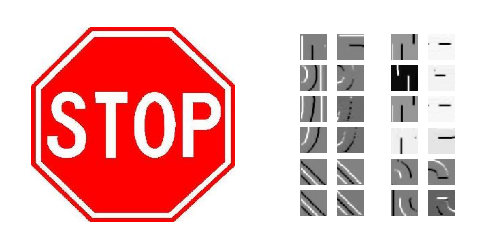
\includegraphics[scale=0.65]{images/gradients_patch.png}
	\caption{Stop-Schild und Gradienten um einige der gefundenen \textit{keypoints}.}
	\label{img:gradients}
\end{figure}

\subsection{Autoencoder Modell in TensorFlow}

Zur Implementierung des Autoencoders wurde TensorFlow verwendet. TensorFlow ist ein DeepLearning Framework und bietet Schnittstellen in diversen Sprachen an. Neben OpenCL wird auch NVIDIAs CUDA unterstützt, sodass TensorFlow Programme automatisch von Grafikkarten profitieren können, ohne das der Entwickler diese explizit berücksichtigen muss. Für diese Umsetzung eines Autoencoders wurde Python und das Projekt \textit{libsdae-autoencoder-tensorflow}\footnote{https://github.com/rajarsheem/libsdae-autoencoder-tensorflow} von Rajarshee Mitra genutzt. Unter Berücksichtigung der bekannten Parameter aus dem Konzept, ergibt sich die folgende Definition eines Modells:

\lstset{language=Python}
\begin{lstlisting}
from deepautoencoder import StackedAutoEncoder
import cv2
import numpy
import featureExtractor

imagePaths = []

features = featureExtractor.extractAll(imagePaths)
index = numpy.random.rand(features.shape[0]) < 0.8
train = features[index]
test = features[~index]

model = StackedAutoEncoder(
  dims=[3042, 1024, 512, 128, 36],
  activations=['relu', 'relu', 'relu', 'relu', 'relu'], 
  epoch=[1000, 1000, 700, 700, 500], 
  loss='rmse', 
  lr=0.02, 
  batch_size=100
)

model.fit(train)
result = model.transform(test)
\end{lstlisting}

In Zeile 8 wird die bereits eingeführte Funktion \textit{extractAll} genutzt, um alle Features der Bilder, die in \textit{imagePaths} enthalten sind, zu gewinnen. Diese werden in der Zeile 10 bzw. 11 in eine Test- und Trainingsmenge aufgeteilt, wobei \todo{erstere 80\% und letztere 20\% der Bilder enthält}.
In den Zeilen 12 bis 19 findet die Definition des Autoencoders statt. Der \textit{StackedAutoEncoder} entstammt hierbei dem Eingangs erwähnten Projekt von Rajarshee Mitra. In \textit{dims} wird die Menge der Schichten des Encoder-Teils durch eine Liste von Ganzzahlen dargestellt: Eine Zahl steht für die Anzahl der Neuronen pro Schicht. Hier wird davon ausgegangen, dass benachbarte Schichten voll verbunden sind. Der Decoder-Teil ist umgekehrt aufgebaut, daher leitet sich dieser aus der Encoder-Definition ab und muss nicht notiert werden. Folglich werden in \textit{activations} die Aktivierungsfunktion auch nur einmal notiert. Die Abkürzung \textit{relu} steht hier für Rectified Linear Unit (ReLU). \todo{Die verwendete Aktivierungsfunktion zwischen den Schichten wurde in dem Paper das als Basis des Autoencoders diente nicht erwähnt.} ReLU wird in vielen Netzen verwendet, die Funktion ist recht simpel: Negative Werte sowie Gradienten die gegen unendlich gehen, wie beispielsweise bei der Sigmoidfunktion möglich, werden vermieden. Da über die Anzahl der Iterationen die pro Autoencoder-Paar im Training ausgeführt werden soll, keine Angaben vorliegen, wurden hier Zahlen getestet die üblich sind. Durch eine Variation der Iteration in mehreren Testläufen kann eine Zahl ermittelt werden, die ein gutes Verhältnis von Fehlerrate zu Ausführungszeit bietet: Gerade in den Ersten schichten des Encoders, bzw. den Letzten des Decoders, sind erheblich mehr Verbindungen vorhanden. In Zeile 17 wird unter \textit{loss} die die Metrik definiert, mit der der Fehler bei Rekonstruktion gemessen wird. \textit{rmse} steht für \textit{root-mean-square error} und ist somit der gemittelte quadratische Fehler. Die Lernrate wird hier mit \textit{lr} bezeichnet und wurde entsprechend des konzipierten Autoencoders auf 2\% gesetzt.
In Zeile 22 wird \textit{fit} aufgerufen um das Modell mit den \textit{train} Features zu trainieren. Hierbei kann optional durch \textit{print\textunderscore step} angegeben werden, nach wie vielen Iterationen im Training pro Autoencoder-Paar die Fehlerrate ausgegeben werden soll.
Anschließend wird der Autoencoder genutzt um die Testdaten einmal zu komprimieren und wieder zu rekonstruieren. Auf diese Weise kann \textit{result} zum Beispiel genutzt werden, um eine Beurteilung durch einen Menschen zu ermöglichen: Handelt es sich wie hier um Bilder von Gradienten, können so Original und Rekonstruktion nebeneinander gestellt als Bild gespeichert werden. Für praktische Anwendung ist es interessanter, nur den Encoder-Teil anzuwenden, um auf Basis der komprimierten Darstellung eine Klassifikation oder Speicherung zu ermöglichen.  